\Chapter{A minta alkalmazás}

A mintaalkalmazás egy könyvtár adatainak kezelését valósítja meg online felületen. Könyvek böngészésén és kölcsönzésén kívül lehetősége van a felhasználónak könyveket értékelni, hozzászólásokat írni, listákat létrehozni, könyvjelzőket kezelni, valamint új könyvekre igényt leadni. Ebben a fejezetben az alkalmazás által nyújtott funkciók részletes bemutatásáról, valamint azok megvalósításáról lesz szó.

\Section{Szerepkörök, használati esetek}

Az alkalmazás használati eset (\textit{use-case}) diagramja \aref{fig:use-case}. ábrán található.

\begin{figure}[h]
	\centering
	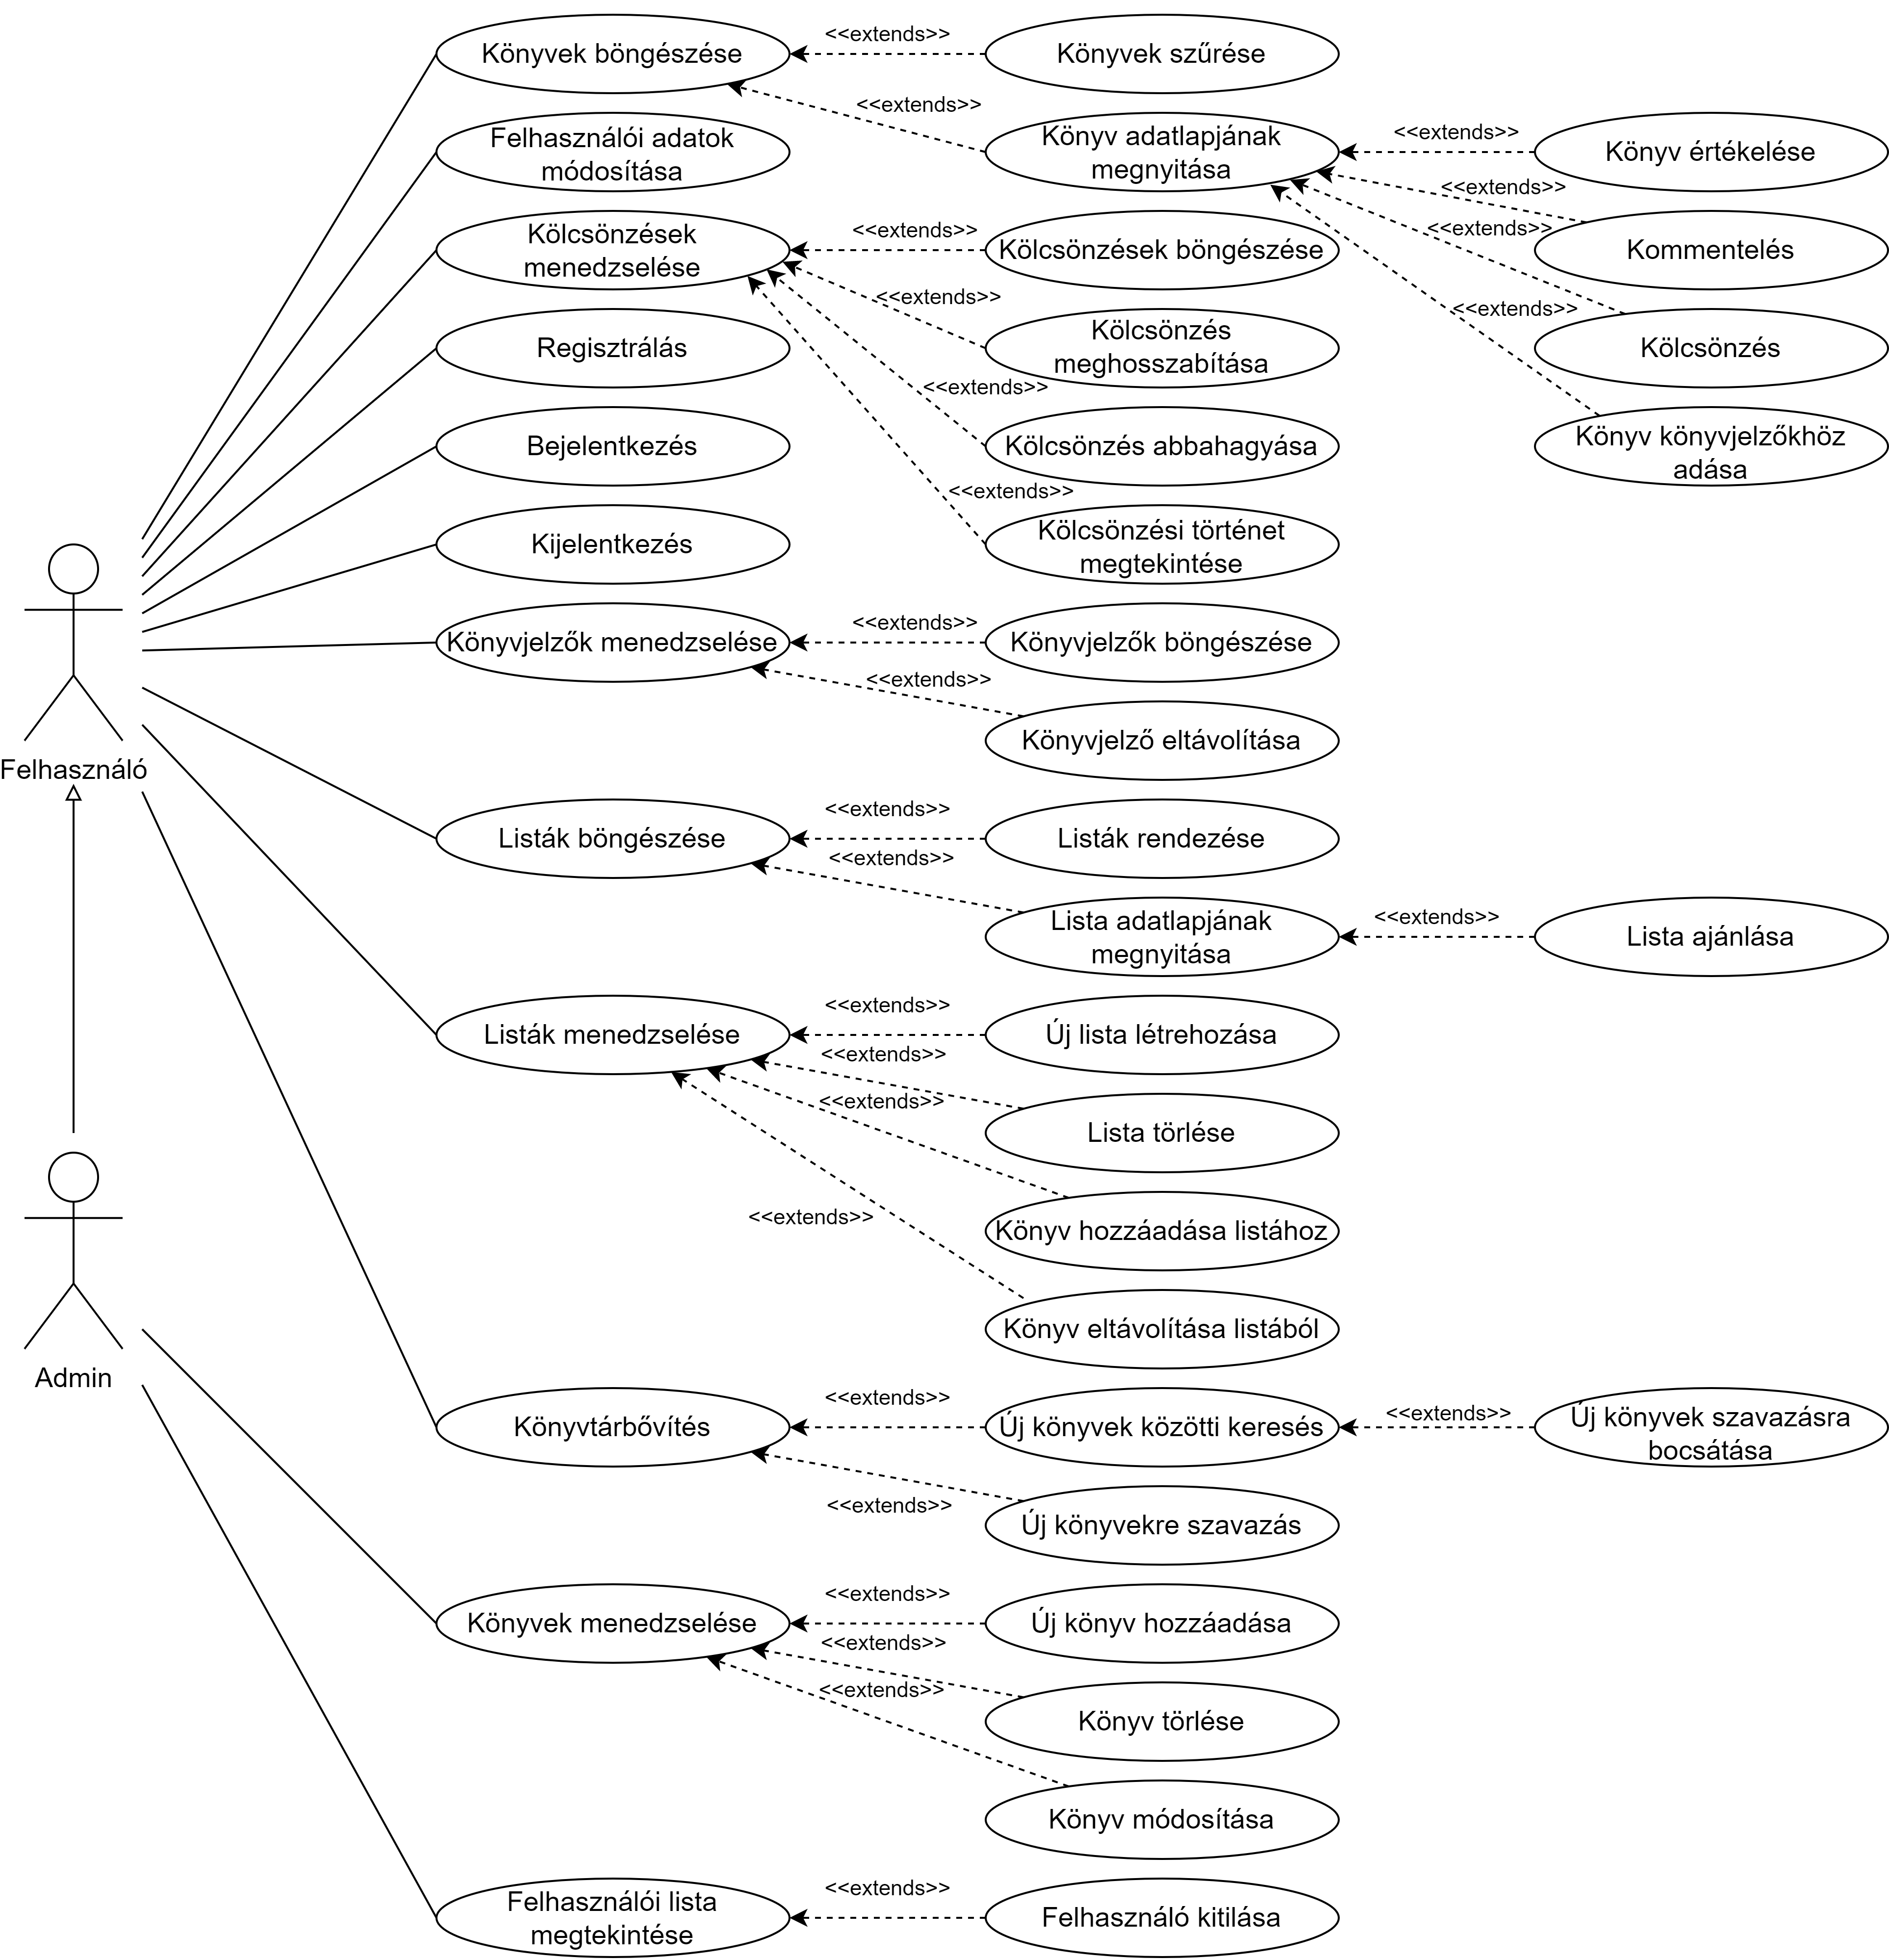
\includegraphics[scale=0.6]{images/graphlibrary-usecase-better.png}
	\caption{Az alkalmazás használati esetei}
	\label{fig:use-case}
\end{figure}

Egy átlagos felhasználó az alkalmazásban az alábbiakban felsorolt funkciókat tudja igénybe venni.
\begin{itemize}
    \item Felhasználói fiókkal kapcsolatos funkciók: regisztrálás, bejelentkezés, kijelentkezés, felhasználói adatok módosítása.
    \item Könyvkereséssel kapcsolatos funkciók: könyvek böngészése, könyvek szűrése, \\ könyvek adatlapjának megnyitása.
    \item A könyvek adatlapján igénybe vehető funkciók: könyvek értékelése, megjegyzés írása, könyv kikölcsönözése, könyv könyvjelzőkhöz adása, könyv eltávolítása.
    \item Kölcsönzésekkel kapcsolatos funkciók: kölcsönzések böngészése, kölcsönzések \\ meghosszabbítása, könyvek visszavitele, felhasználó kölcsönzési történetének \\ megtekintése.
    \item Könyvjelzőkkel kapcsolatos funkciók: könyvjelzők böngészése, könyvjelzők eltávolítása.
    \item Listák böngészésével kapcsolatos funkciók: listák böngészése, rendezése, listák adatlapjának megtekintése, listák ajánlása.
    \item Saját listákkal kapcsolatos funkciók: új lista létrehozása, lista törlése, könyv listához adása, könyv eltávolítása a listából.
    \item Könyvtárbővítéssel kapcsolatos funkciók: lehetséges könyvek közötti keresés, azok szavazásra bocsátása, szavazatra bocsátott könyvekre szavazás.
\end{itemize}

Adminisztrátori jogosultságú felhasználó az alkalmazásban az alábbi funkciókat tudja igénybe venni.
\begin{itemize}
    \item Felhasználókkal kapcsolatos funkciók: felhasználói lista megtekintése, felhasználók kitiltása.
    \item Könyvekkel kapcsolatos funkciók: új könyv könyvtárhoz adása, meglévő könyvek módosítása, könyvek törlése.
\end{itemize}

\Section{Funkciók, műveletek}

Ebben az alfejezetben bemutatásra kerül, hogy milyen funkciókkal van felruházva a mintaalkalmazás. A bemutatás az alkalmazás menüpontjain keresztül fog zajlani.

\subsection{Books menüpont}

A \textit{Books} menüpont az alkalmazás központi része (\ref{fig:books}. ábra). Innen érheti el a felhasználó a könyvtárban található könyvek adatait. A menüpont megnyitásakor az oldal közepén megjelennek a könyvtárban található könyvek. Egyszerre csak egy adott számú könyv jelenik meg, további könyveket a találatok alatt lévő lapszámozás funkció segítségével lehet elérni. A nyilakra kattintva egy-egy oldallal az adott irányba lehet lépni, míg egy adott számra kattintva az azzal megegyező sorszámú találatoldal fog megjelenni.

\begin{figure}[h]
\centering
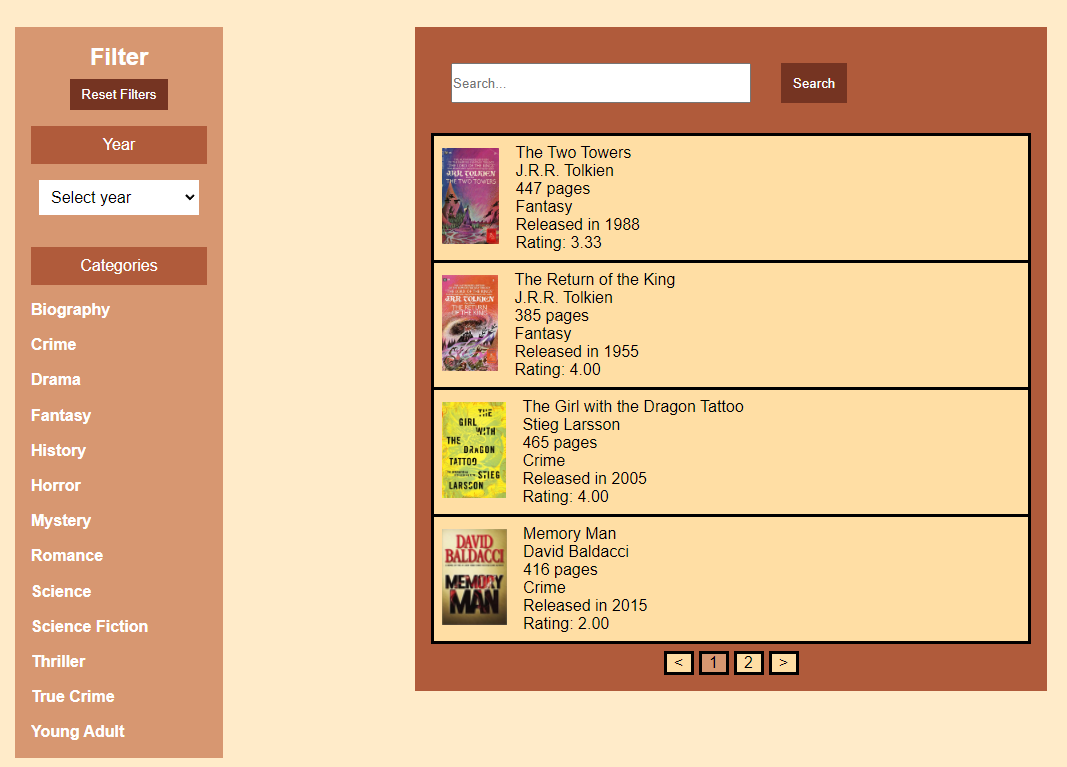
\includegraphics[scale=0.5]{images/application/books.png}
\caption{A Books menüpont}
\label{fig:books}
\end{figure}

A megjelenő könyveket lehetősége van a felhasználónak szűrni. A könyvek felett található keresési mezőbe beírhatja a felhasználó egy könyv címét, vagy címének egy részletét, és ekkor csak a keresésnek megfelelő könyvek fognak megjelenni a listában. Ezen kívül lehetősége van még a felhasználónak a könyvektől balra található felületen megjelenési év, valamint kategória szerint is szűrni a találatokat. Ez a három szűrési lehetőség egyszerre is használható.

Minden megjelenő könyvhöz tartozik egy rövid összefoglaló. Ebben az összefoglalóban megtudhatja a felhasználó az adott könyv címét, a szerzőjét, oldalainak számát, kategóriáját, megjelenési évét, borítója, valamint a más felhasználók értékelésének átlagát. Egy összefoglalóra kattintva megjelenik az adott könyv adatlapja (\ref{fig:bookcard}. ábra).

Egy könyv adatlapját megnyitva megjelennek a könyv adatai, úgy mint: 
\begin{itemize}
    \item cím,
    \item szerző,
    \item rövid tartalmi összefoglaló,
    \item hossz,
    \item kategória,
    \item megjelenési év,
    \item értékelések átlaga,
    \item könyvtári példányok száma.
\end{itemize}

\begin{figure}[h]
    \centering
    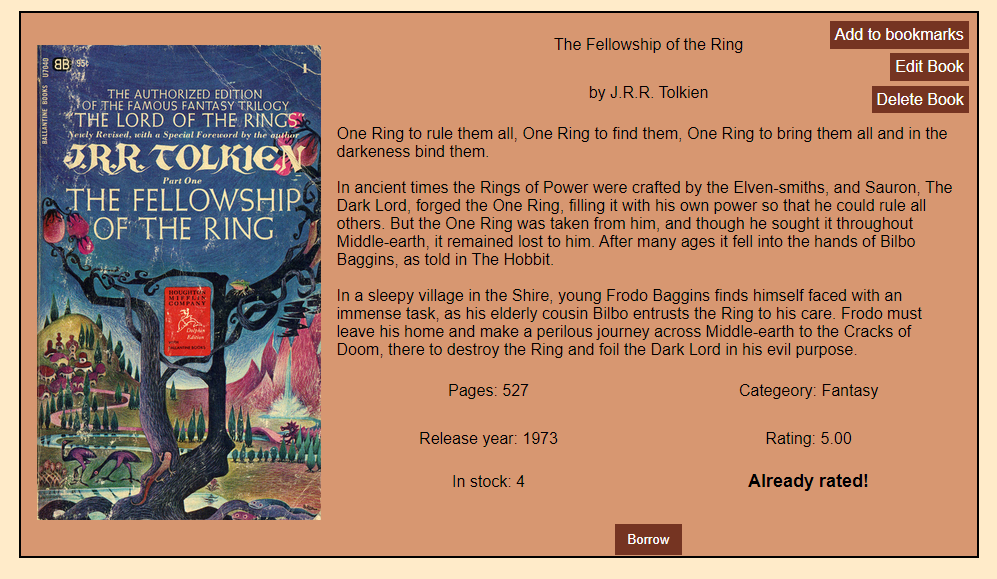
\includegraphics[scale=0.55]{images/application/bookcard.png}
    \caption{Egy könyv adatlapja}
    \label{fig:bookcard}
\end{figure}

Az adatlap alatt más felhasználók által írt kommenteket találhat a felhasználó. Egy kommentnél az alábbi információk jelennek meg:
\begin{itemize}
    \item a kommentelő neve,
    \item a komment írásának dátuma,
    \item a komment szöveges tartalma.
\end{itemize}
Bejelentkezés nélkül a felhasználónak csak az adatlap megtekintésére van lehetősége. Egy bejelentkezett felhasználó számára az alábbi funkciók is elérhetővé válnak.
\begin{itemize}
    \item Az értékelések alatt lehetősége van egy regisztrált felhasználónak a könyv értékelésére 1 és 5 közötti értékkel.
    \item  Az adatlap jobb felső sarkában a felhasználó a könyvjelzőihez adhatja a könyvet, vagy ha már ott volt, akkor eltávolíthatja azt onnan.
    \item  Az adatlap alján lehetősége van a felhasználónak az adott könyv kikölcsönzésére, amennyiben a könyv készleten van.
    \item  Az adatlap alatt írhat saját kommentet is a felhasználó.
\end{itemize}
Admin jogosultsággal rendelkező felhasználónak a könyv adatlapról lehetősége van még ezeken kívül a könyvet szerkeszteni, illetve törölni.

\subsection{Lists menüpont}

A \textit{Lists} menüpontban lehetősége van a felhasználónak más felhasználók által készített listák megtekintésére, valamint saját listák menedzselésére.

A \textit{Browse Lists} almenüpontra kattintva megjelennek a felhasználók által készített listák. A \textit{Books} menüponthoz hasonlóan itt a lapszámozás funkció segítségével válthat a felhasználó a listák között. A listákat lehetősége van a felhasználónak ajánlások, illetve létrehozási dátum szerint rendezni. Minden listához tartozik egy összefoglaló, ami az alábbiakat tartalmazza:
\begin{itemize}
    \item a lista neve,
    \item a listában levő könyvek száma,
    \item az ajánlások száma,
    \item a lista létrehozásának dátuma.
\end{itemize}
Egy lista összefoglalójára kattintva megjelenik a lista adatlapja (\ref{fig:listcard}. ábra).

\begin{figure}[h]
    \centering
    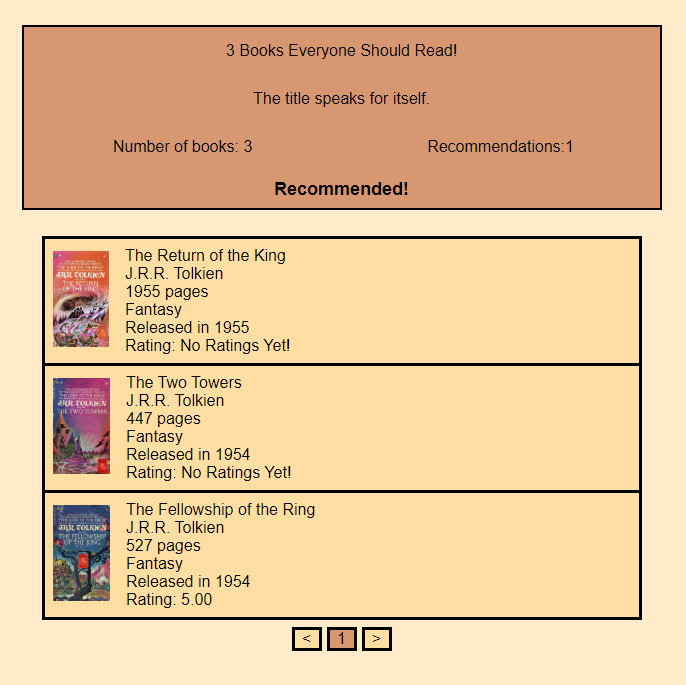
\includegraphics[scale=0.65]{images/application/listcard.png}
    \caption{Egy lista adatlapja}
    \label{fig:listcard}
\end{figure}

\noindent A lista adatlapján az alábbiak szerepelnek:
\begin{itemize}
    \item a lista neve,
    \item a lista leírása,
    \item listában levő könyvek száma,
    \item az ajánlások száma.
\end{itemize}

Az adatlap alatt láthatja a felhasználó, hogy pontosan mely könyvek vannak a listában. Bejelentkezett felhasználónak lehetősége van a lista ajánlására.

A \textit{New List} menüpontban a felhasználó egy listanév és egy leírás megadásával saját listát hozhat létre. A felhasználó a saját listáit a \textit{Delete List} menüpontban törölheti.

Az \textit{Add Books To List} menüpontban lehetősége van a felhasználónak kiválasztania egyet a listái közül. Egy lista kiválasztása utána a \textit{Books} menüpont felülete jelenik meg annyi különbséggel, hogy minden könyv elemhez tartozik egy \textit{Add} gomb, amivel az adott könyv a listához rendelhető. A \textit{Remove Book From List} menüpontban a lista kiválasztása után megjelennek a listához tartozó könyvek, melyeket a \textit{Remove} gombra kattintva lehet eltávolítani az adott listából.

\subsection{Expand menüpont}

Az \textit{Expand} menüpont lehetőséget nyújt a felhasználók számára, hogy a könyvtárban még nem található könyvekkel bővítsék a könyvtár készletét. 

Az \textit{Add} almenüpontban lehetősége van a felhasználónak cím, író és kategória szerint keresni a Google Books katalógusában. Keresés után megjelennek a találatok, melyekhez tartozik egy-egy rövid összefoglaló, amely az alábbi adatokat tartalmazza:
\begin{itemize}
    \item cím,
    \item író,
    \item oldalszám,
    \item kategória,
    \item megjelenési év,
    \item tartalmi összegzés (kattintás után).
\end{itemize}
Minden találathoz tartozik egy \textit{Add} gomb, amire ha rákattint a felhasználó, akkor a könyv szavazásra bocsátásra kerül.

A \textit{Vote} almenüpontban lehetősége van a felhasználónak szavazásra bocsátott könyvekre szavazni. Ha egy könyv elég szavazatot gyűjt, akkor az hozzáadódik a könyvtárhoz (\ref{fig:expand}. ábra).

\begin{figure}[h]
    \centering
    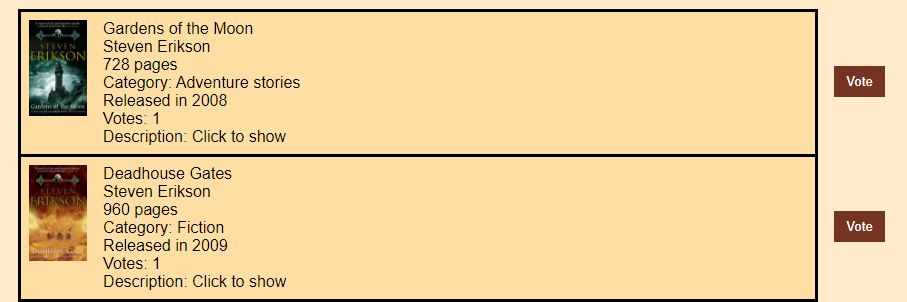
\includegraphics[scale=0.5]{images/application/expand.png}
    \caption{Bővítés menüpont -- Szavazás funkció}
    \label{fig:expand}
\end{figure}

\subsection{Borrowings menüpont}

A \textit{Borrowings} menüpontban tudja a felhasználó megtekinteni a jelenlegi kölcsönzéseit. A könyvek a rövid összefoglaló formájukban jelennek meg. Minden megjelenő könyvtől jobbra találhatóak a kölcsönzéssel kapcsolatos információk, illetve lehetőségek (\ref{fig:borrowings}. ábra). 

\begin{figure}[h]
    \centering
    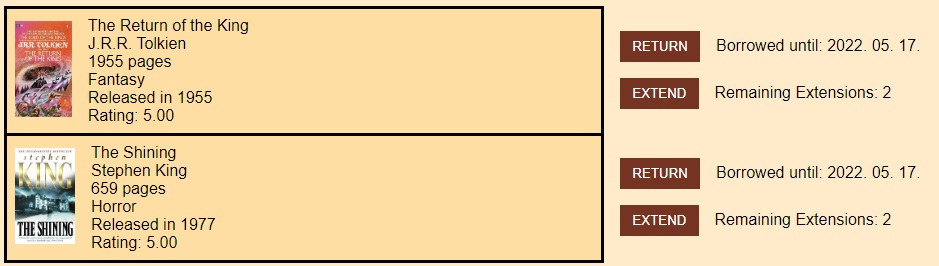
\includegraphics[scale=0.6]{images/application/borrowings.png}
    \caption{Kölcsönzések menüpont}
    \label{fig:borrowings}
\end{figure}

Egy könyv kikölcsönzése alapvetően 30 napra szól. Ezt az időtartamot a felhasználónak kétszer van lehetősége meghosszabbítani, mindegyik hosszabbítás 30 napot ad a teljes időtartamhoz, tehát egy felhasználó egy könyvet maximum 90 napig tarthat magánál. Azt, hogy hány hosszabbítási lehetősége van a felhasználónak, és hogy meddig tart a kölcsönzési határidő, a könyvtől jobbra található részen láthatja a felhasználó. Az \textit{Extend} gombra kattintva megtörténik a hosszabbítás, a \textit{Return} gombra kattintva pedig a felhasználó visszaadja a könyvet a könyvtárnak. 

\subsection{Bookmarks menüpont}

A \textit{Bookmarks} menüpontban megtekintheti a felhasználó a könyvjelzőit. A könyvek a rövid összefoglaló formájukban jelennek meg. Minden könyvhöz tartozik egy \textit{Remove} gomb, amivel a felhasználó eltávolíthatja a könyvet a könyvjelzők közül (\ref{fig:bookmarks}. ábra).

\begin{figure}[h]
    \centering
    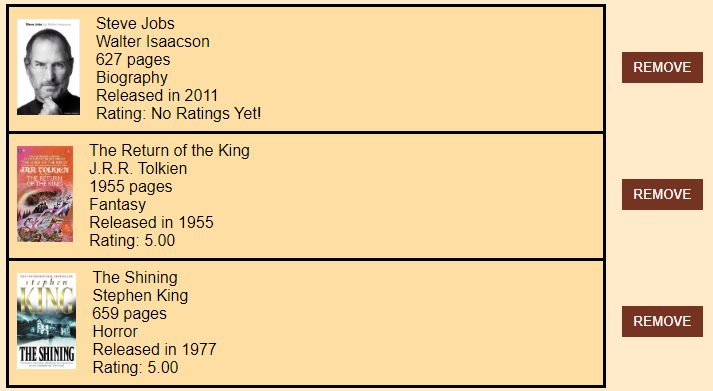
\includegraphics[scale=0.65]{images/application/bookmarks.png}
    \caption{Könyvjelzők menüpont}
    \label{fig:bookmarks}
\end{figure}

\subsection{Admin menüpont}

Az \textit{Admin} menüponthoz csak az adminisztrátor jogosultsággal rendelkező felhasználóknak van hozzáférési joga. 

Az \textit{Add New Book} gombra kattintva megjelenik egy űrlap, amelyen meg tudja adni az adminisztrátor az új könyv címét, szerzőjét, rövid tartalmi összegzését, hosszát, kategóriáját, megjelenési évét, borítóját, és hogy hány darab van a könyvből készleten. Az \textit{Add Book} gombra kattintva az űrlapon megadott könyv hozzáadódik a könyvtárhoz (\ref{fig:newbook}. ábra).

\begin{figure}[h]
    \centering
    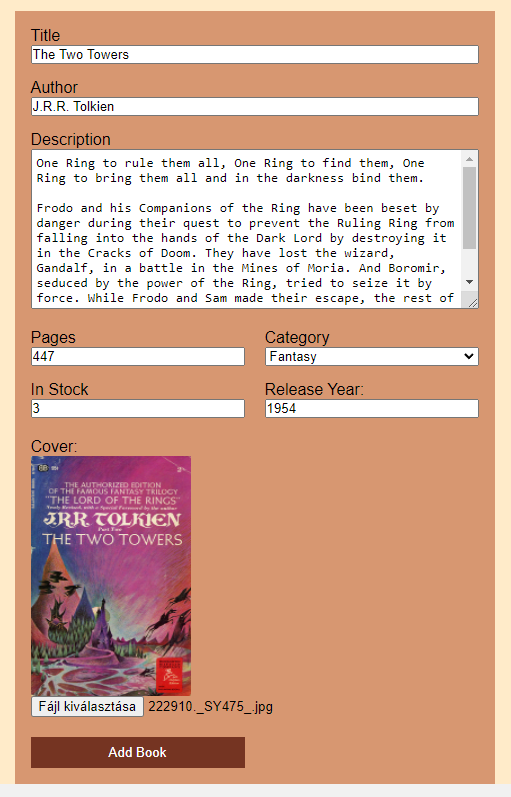
\includegraphics[scale=0.6]{images/application/newbook.png}
    \caption{Új könyv hozzáadása}
    \label{fig:newbook}
\end{figure}

A \textit{User List} gombra kattintva megjelenik az összes felhasználó neve és email címe (\ref{fig:userlist}. ábra). A \textit{Ban user} gombra kattintva lehetősége van az adminisztrátornak egy felhasználó végleges kitiltására.

\begin{figure}[h]
    \centering
    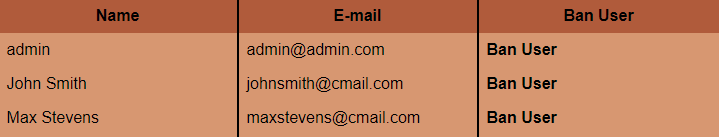
\includegraphics[scale=0.6]{images/application/userlist.png}
    \caption{Felhasználói lista}
    \label{fig:userlist}
\end{figure}

\subsection{Signup menüpont}

A \textit{Signup} menüpontban hozhat létre a felhasználó saját felhasználói fiókot. Egy ilyen fiók szükséges ahhoz, hogy az alkalmazás funkcióinak többsége igénybe vehető legyen. A regisztrációhoz meg kell adni egy nevet, egy egyedi email címet és egy jelszót. Már foglalt email cím megadása esetén a felhasználó hibaüzenetet kap.

\subsection{Login menüpont}

A \textit{Login} menüpontban léphet be a felhasználó a létrehozott felhasználói fiókjába helyes email cím és jelszó kombináció megadása után. Hibás bejelentkezési adatok esetén a felhasználó hibaüzenetet kap.

\subsection{Profile menüpont}

A \textit{History} gombra kattintva megtekintheti a felhasználó, hogy milyen korábbi kölcsönzései voltak.

A \textit{Change User Data} gombra kattintva lehetősége van a felhasználónak a nevét, jelszavát és/vagy email címét megváltoztatni a jelenlegi jelszó megadása után. Hibás adatok esetén a felhasználó hibaüzenetet kap.

\Section{Az alkalmazás architektúrája}

Az alkalmazás architektúrájának fő elemeit \aref{fig:graphlibrary_architecture}. ábra foglalja össze.

\begin{figure}[h]
   \centering
   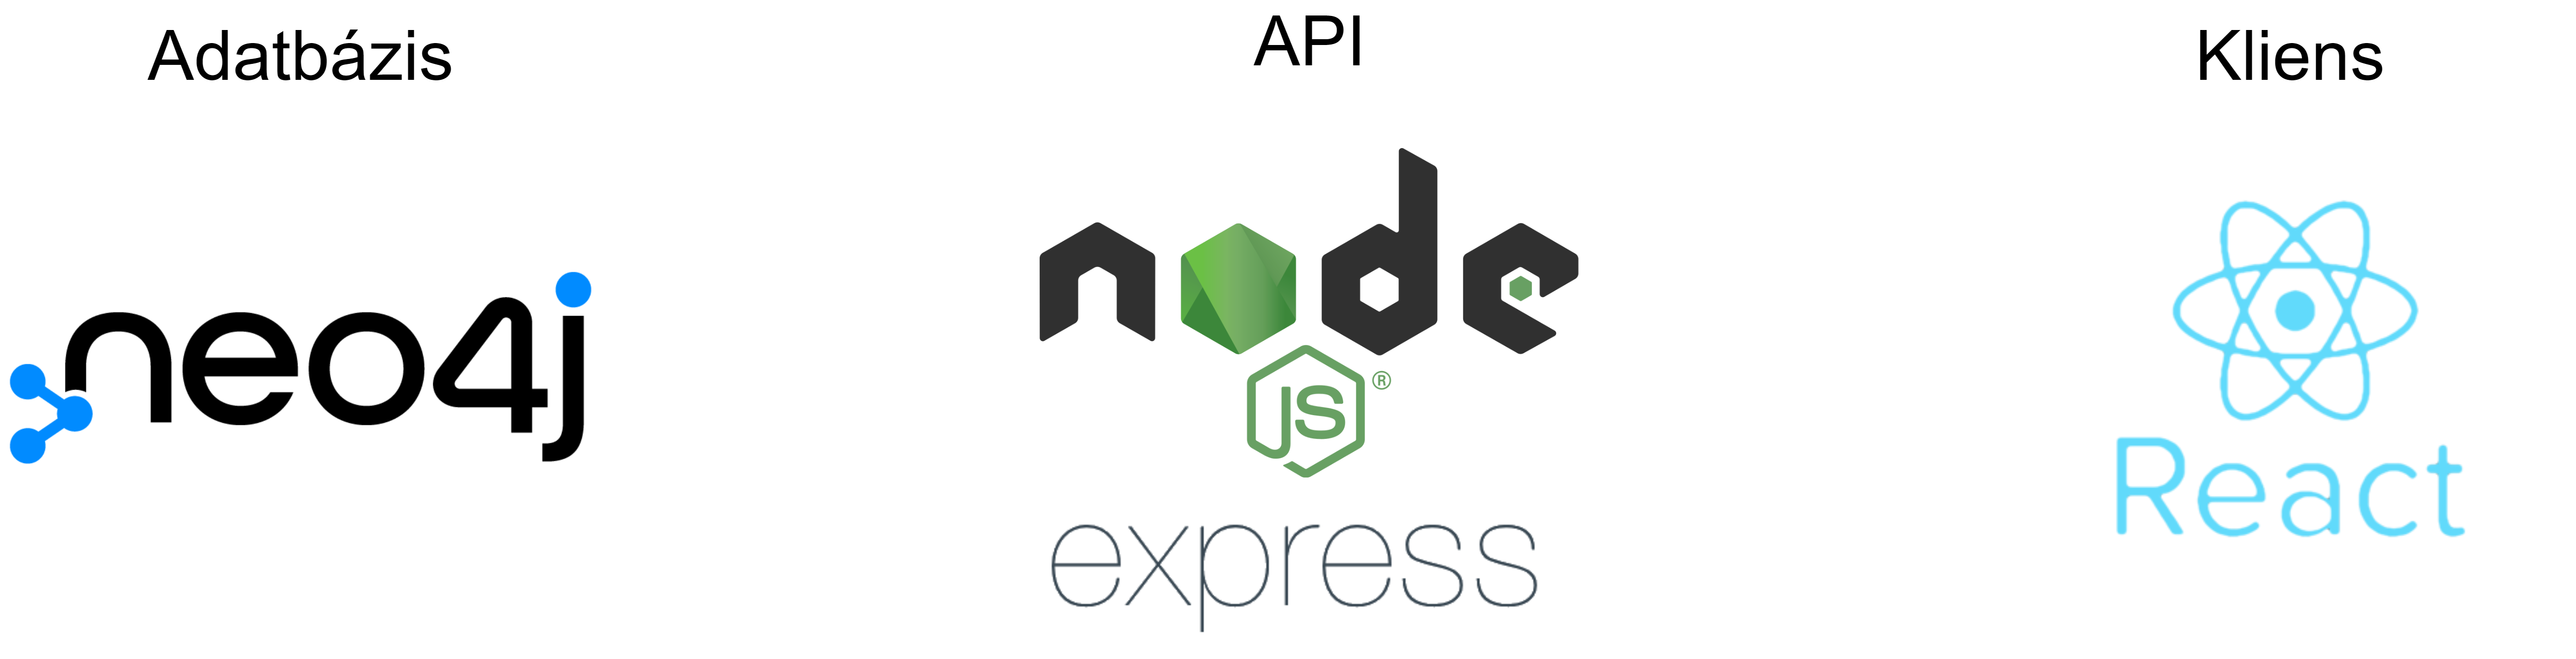
\includegraphics[scale=0.3]{images/graphlibrary_architecture.png}
   \caption{Az alkalmazás architektúrájának sematikus ábrája}
   \label{fig:graphlibrary_architecture}
\end{figure}

A kliens a React könyvtár segítségével valósul meg. Az adatok a Neo4j gráfadatbázisban kerülnek tárolásra. A kettő közötti kommunikációt a NodeJS és az Express keretrendszer teszi lehetővé.

\Section{Az alkalmazás API-ja}

Ebben az alfejezetben található az API tömör leírása. Az API részletes, OpenAPI szabvány szerinti leírása külön (a \texttt{graph-library-api.yaml}) fájlban olvasható.

A tervezés során szempont volt a REST architekturális stílus alkalmazása. A következőkben az API bemutatásánál a jellegzetességekre, döntési pontok indoklására kerül majd sor. (Az egyszerűbb, következetesen adódó esetek különösebb részletezése nem tünt szükségesnek.)

\subsection{Könyvekkel kapcsolatos operációk}

\Aref{tab:book}. táblázatban láthatjuk a könyvekhez kapcsolódó műveleteket. Ennek egy érdekesebb pontja több könyv adatainak visszaadása az azonosítók alapján. Ez egy GET típusú kérés, amelynél viszont paraméterként szerepelnie kell a könyvek azonosítóinak listájának. Mivel az egyidejűleg lekérdezésre kerülő könyvek száma lehetővé tette, ezért ez az útvonalban került megadásra.

\renewcommand\tabularxcolumn[1]{m{#1}}
\begin{center}
\begin{table}[h]
\caption{Book operációk}
\label{tab:book}
\smallskip
\begin{tabularx}{\textwidth}{ |l|c|Y|Y| } 
 \hline
 \multicolumn{1}{|c|}{\texttt{Útvonal}} & \texttt{Metódus} & \texttt{Paraméterek} & \texttt{Feladat} \\ 
 \hhline{|=|=|=|=|}
 /book & POST & Könyv objektum & Új könyv létrehozása  \\ 
 \hline
 /book & GET & Keresési feltételek, Pagination adatok & Könyvek visszaadása  \\ 
 \hline
 /book & DELETE & Könyv ID & Könyv törlése  \\ 
 \hline
 /book & PUT & Könyv objektum & Könyv módosítása  \\ 
 \hline
 /book/list/\{listOfIds\} & GET & Könyv ID-k listája, Pagination adatok & Könyvek visszaadása  \\ 
 \hline
 /book/\{bookId\} & GET & Könyv ID & ID-nek megfelelő könyv visszaadása  \\ 
 \hline
 /book/rate & POST & Könyv és Felhasználó ID, Értékelés & Új értékelés hozzáadása  \\ 
 \hline
\end{tabularx}
\end{table}
\end{center}

\subsection{Kommentekkel kapcsolatos operációk}

A kommentekhez kapcsolódó műveleteket \aref{tab:comment}. táblázatban láthatjuk. Mivel a megjegyzések utólagos szerkesztésére a rendszer (az aktuális változat tervei szerint) nem ad lehetőséget, ezért elegendő volt csak a könyvhöz tartozó kommentek lekérdezését és új komment létrehozását biztosítani az API-n keresztül.

\begin{center}
\begin{table}[h]
\caption{Comment operációk}
\label{tab:comment}
\smallskip
\begin{tabularx}{\textwidth}{ |l|c|Y|Y| } 
 \hline
 \multicolumn{1}{|c|}{\texttt{Útvonal}} & \texttt{Metódus} & \texttt{Paraméterek} & \texttt{Feladat} \\ 
 \hhline{|=|=|=|=|}
 /comment/\{bookId\} & GET & Könyv ID & Könyvhöz tartozó kommentek visszaadása  \\ 
 \hline
 /comment & POST & Komment objektum & Új komment létrehozása  \\ 
 \hline
\end{tabularx}
\end{table}
\end{center}

\subsection{Listákkal kapcsolatos operációk}

A listákhoz tartozó műveleteket \aref{tab:list}. táblázat foglalja össze. A könyvekhez és kommentekhez hasonlóan, az API nem teljes körű olyan tekintetben, hogy például az ajánlásokhoz nem biztosít minden CRUD műveletet. Ez ez esetben sem következetlenség, hanem a specifikált funkcionalitás nem tette szükségessé ezen végpontok kialakítását.

\begin{center}
\begin{table}[h]
\caption{List operációk}
\label{tab:list}
\smallskip
\begin{tabularx}{\textwidth}{ |l|c|Y|Y| } 
 \hline
 \multicolumn{1}{|c|}{\texttt{Útvonal}} & \texttt{Metódus} & \texttt{Paraméterek} & \texttt{Feladat} \\ 
 \hhline{|=|=|=|=|}
 /list & POST & Lista objektum & Új lista létrehozása  \\ 
 \hline
 /list & GET & Pagination információk, Rendezési sorrend & Lista visszaadása  \\ 
 \hline
 /list & DELETE & Lista ID & Lista törlése  \\ 
 \hline
 /list/user/\{userId\} & GET & Felhasználó ID & Felhasználó listáinak visszaadása  \\ 
 \hline
 /list/\{listId\} & GET & Könyv objektum & ID-nek megfelelő lista visszaadása  \\ 
 \hline
 /list/book & POST & Könyv ID, Lista ID & Könyv listához adása  \\ 
 \hline
 /list/book & DELETE & Könyv ID, Lista & Könyv törlése listából  \\ 
 \hline
 /list/recommendation & POST & Lista ID & Új ajánlás hozzáadása  \\ 
 \hline
\end{tabularx}
\end{table}
\end{center}

\subsection{Bővítéssel kapcsolatos operációk}

A könyvállomány bővítéséhez kapcsolódó műveleteket \aref{tab:expand}. táblázatban láthatjuk. Ez egyúttal tartalmazza a szavazáshoz szükséges végpontot is.

\begin{center}
\begin{table}[H]
\caption{Expand operációk}
\label{tab:expand}
\smallskip
\begin{tabularx}{\textwidth}{ |l|c|Y|Y| } 
 \hline
 \multicolumn{1}{|c|}{\texttt{Útvonal}} & \texttt{Metódus} & \texttt{Paraméterek} & \texttt{Feladat} \\ 
 \hhline{|=|=|=|=|}
 /expand & POST & Könyv objektum, Felhasználó ID & Új potenciális könyv létrehozása  \\ 
 \hline
 /expand & GET & Pagination információk & Potenciális könyvek visszaadása  \\ 
 \hline
 /expand & DELETE & Könyv ID & Potenciális könyv eltávolítása  \\ 
 \hline
 /expand/vote & POST & Könyv ID, Felhasználó ID & Új szavazás hozzáadása  \\ 
 \hline
\end{tabularx}
\end{table}
\end{center}

\subsection{Kölcsönzésekkel kapcsolatos operációk}

A kölcsönzés esetében \aref{tab:borrow}. táblázatban látható műveletek érhetők el. A kölcsönzést leíró objektum átadása esetén a felhasználói azonosítónak nem szükséges szerepelnie az útvonalban.

\begin{center}
\begin{table}[h]
\caption{Borrow operációk}
\label{tab:borrow}
\smallskip
\begin{tabularx}{\textwidth}{ |l|c|Y|Y| }
 \hline
 \multicolumn{1}{|c|}{\texttt{Útvonal}} & \texttt{Metódus} & \texttt{Paraméterek} & \texttt{Feladat} \\ 
 \hhline{|=|=|=|=|}
 /borrow/\{userId\} & GET & Felhasználó ID & Felhasználó kölcsönzéseinek visszaadása\\ 
 \hline
 /borrow & POST & Kölcsönzés objektum & Új Kölcsönzés létrehozása  \\ 
 \hline
 /borrow & DELETE & Kölcsönzés objektum & Kölcsönzés törlése \\ 
 \hline
 /borrow/extend & POST & Kölcsönzés objektum & Kölcsönzés meghosszabbítása \\ 
 \hline
\end{tabularx}
\end{table}
\end{center}

\subsection{Könyvjelzőkkel kapcsolatos operációk}

A könyvjelzők műveleteinek áttekintését \aref{tab:bookmarks}. táblázatban láthatjuk.

\begin{center}
\begin{table}[h]
\caption{Bookmarks operációk}
\label{tab:bookmarks}
\smallskip
\begin{tabularx}{\textwidth}{ |l|c|Y|Y| } 
 \hline
 \multicolumn{1}{|c|}{\texttt{Útvonal}} & \texttt{Metódus} & \texttt{Paraméterek} & \texttt{Feladat} \\ 
 \hhline{|=|=|=|=|}
 /bookmarks/\{userId\} & GET & Felhasználó ID & Felhasználó könyvjelzőinek visszaadása\\ 
 \hline
 /bookmarks & POST & Könyvjelző objektum & Új könyvjelző létrehozása  \\ 
 \hline
 /bookmarks & DELETE & Könyvjelző objektum & Könyvjelző törlése \\ 
 \hline
\end{tabularx}
\end{table}
\end{center}

\subsection{Felhasználókkal kapcsolatos operációk}

A felhasználók kezeléséhez tartozó műveleteket \aref{tab:user}. táblázat foglalja össze. A módosítással és törléssel kapcsolatos adatok a PUT és a DELETE kérés paramétereibe kerültek. Alternatívaként felvetődött a felhasználói azonosító útvonalban történő megadása is.

\begin{center}
\begin{table}[h]
\caption{User operációk}
\label{tab:user}
\smallskip
\begin{tabularx}{\textwidth}{ |l|c|Y|Y| } 
 \hline
 \multicolumn{1}{|c|}{\texttt{Útvonal}} & \texttt{Metódus} & \texttt{Paraméterek} & \texttt{Feladat} \\ 
 \hhline{|=|=|=|=|}
 /user & POST & Felhasználó objektum & Új felhasználói fiók létrehozása  \\ 
 \hline
 /user & GET & - & Felhasználók visszaadása  \\ 
 \hline
 /user & PUT & Felhasználó objektum & Felhasználó módosítása  \\ 
 \hline
 /user & DELETE & Felhasználó ID & Felhasználói fiók törlése  \\ 
 \hline
 /user/login & POST & Bejelentkezési adatok & Felhasználói fiókba való bejelentkezés \\ 
 \hline
\end{tabularx}
\end{table}
\end{center}

\subsection{Kölcsönzési történettel kapcsolatos operációk}

\Aref{tab:historyborrow}. táblázat a kölcsönzés naplózásához szükséges API végpontok rövid áttekintését mutatja be. Az ehhez tartozó bejegyzések módosítása és törlése nem tünt szükségesnek, így az API kifejezetten egyszerű tudott maradni.

\begin{center}
\begin{table}[h]
\caption{Historyborrow operációk}
\label{tab:historyborrow}
\smallskip
\begin{tabularx}{\textwidth}{ |l|c|Y|Y| } 
 \hline
 \multicolumn{1}{|c|}{\texttt{Útvonal}} & \texttt{Metódus} & \texttt{Paraméterek} & \texttt{Feladat} \\ 
 \hhline{|=|=|=|=|}
 /historyborrow & POST & Felhasználó ID, Könyv ID, Dátum & Kölcsönzés naplózása  \\ 
 \hline
 /historyborrow/\{userID\} & GET & Felhasználó ID, Pagination információk & Kölcsönzése történet visszaadása  \\ 
 \hline
\end{tabularx}
\end{table}
\end{center}

\Section{A kliens alkalmazás}

A kliens alkalmazás a React JavaScript függvénykönyvtárral valósul meg \cite{react}. Ez lehetőséget ad az elemek deklaratív leírására. Komponens alapú szemléletet követ, amellyel így a nagyobb méretű alkalmazások fejlesztése esetében is kezelhető marad a kódbázis.

A komponensek közötti adatcsere property-kkel (úgynevezett \textit{prop}-okkal) valósul meg, például:
\begin{java}
<BookItem
  title={"The Fellowship of the Ring"}
  author={"J.R.R. Tolkien"}
/>
\end{java}
Ebben a példában a \texttt{BookItem} komponens két prop-ot kap (\texttt{title} és \texttt{book}), amiket a komponens később fel tud használni. Ahhoz, hogy ezek elérhetők legyenek, a komponens deklarációjakor be kell állítani, hogy fogadjon propokat:
\begin{java}
const BookItem = (props) => {...}
\end{java}
Ez után például a \texttt{title} prop értékét meg lehet kapni a \texttt{props.title} formában.

Az alkalmazás inicializálása a \texttt{create-react-app} eszközzel történik, aminek a lépései a következők Node package manager esetében:
\begin{itemize}
    \item \texttt{npm install -g create-react-app} parancs futtatása, ami telepíti az eszközt
    \item \texttt{npm init react-app my-app} parancs futtatása, ami inicializálja a React alkalmazást
    \item \texttt{npm start} parancs futtatása, ami elindítja az alkalmazást
\end{itemize}

A \texttt{useState} React Hook segítségével deklarálhatunk úgynevezett állapot változókat. Ezek olyan változók, amelyek a komponens újrarajzolásakor nem veszítik el értéküket. Például:
\begin{java}
const [book, setBook]=useState("The Fellowship of the Ring")
\end{java}
Itt a \texttt{book} a változó, aminek kezdőértéke a "\textit{The Fellowship of the Ring}" sztring. A változó értékét a \texttt{setBook} függvénnyel lehet megváltoztatni:
\begin{java}
setBook("The Two Towers")
\end{java}
Ezzel a változó értéke a "The Two Towers" sztringre változik. A változó értékének változásakor a komponens ez esetben is újrarajzolódik.

\begin{java}
useEffect(() => {
  getBook(bookId).then((data) => {
    setBook(data);
  });
}, [bookId]);
\end{java}
Ebben a \texttt{useEffect}-ben található kód lefut, hogy ha a \texttt{bookId} értéke megváltozik. Futáskor küld egy GET kérést a backend-nek, majd a megkapott adatot átadja a \texttt{book} állapot változónak a \texttt{setBook} függvényt felhasználva. Viszont, ha a kérés elküldése, és a \texttt{setBook} függvény futása között a komponens úgymond lecsatlakozik, tehát például átlépünk egy olyan részére az alkalmazásnak, ahol az adott komponens nincs renderelve, akkor memória szivárgást kapunk. Ennek elkerülése érdekében egy \texttt{cleanup} függvényt kell tennünk a \texttt{useEffect}-be. A \texttt{cleanup} függvény lefut a komponens lecsatlakozásakor. A \texttt{cleanup} függvény alakja:
\begin{java}
return () => {...}
\end{java}
Végeredményben a kiegészített \texttt{useEffect} Hook így fog kinézni:
\begin{java}
useEffect(() => {
  let isActive = true;
  getBook(bookId).then((data) => {
    if (isActive) {
      setBook(data);
    }
  });
  return () => {
    isActive = false;
  };
}, [bookId]);
\end{java}
Ebben az esetben, a \texttt{setBook} csak akkor fut le, hogy ha az \texttt{isActive} változó igaz. A komponens lecsatlakozásakor le fog futni a \texttt{cleanup} függvény, tehát az \texttt{isActive} értéke hamis lesz, tehát a \texttt{setBook} nem fog lefutni, így nem lesz memória szivárgás.

A továbbiakban az alkalmazás komponensei kerülnek bemutatásra.

\subsection{Navigáció}

Az oldalon történő navigáció a React Router segítségével került megvalósításra. A React Rotuer egy React könyvtár, aminek fő célja, hogy segítse a komponensek közötti navigációt. Ehhez először az \texttt{index.js} fájlban az \texttt{App} komponenst \texttt{BrowserRouter} komponensbe kell helyezni:  
\begin{java}
<BrowserRouter>
  <App />
</BrowserRouter>     
\end{java}
Ez után az \texttt{App.js} fájlban a \texttt{Switch} komponensbe lehet írni a különböző \texttt{Route}-ot. A \texttt{Switch} komponens az első egyező útvonalú \texttt{Route}-ot fogja renderelni. A \texttt{Route} szintén egy komponens, amelynek a \texttt{path} paraméterében lehet megadni a kívánt elérési útvonalat, majd a komponensbe el lehet helyezni a renderelni kívánt komponenst, például: 
\begin{java}
<Route path="/books" exact>
  <BooksPage />
</Route>    
\end{java}
Ez azt jelenti, hogy ha az útvonal pontosan \texttt{/books} (az \texttt{exact} miatt), akkor a \\ \texttt{BooksPage} komponens lesz renderelve. Egy útvonal eléréséhez feltételhez is szabható, például így:
\begin{java}
{authCtx.isLoggedIn && (
  <Route path="/profile">
    <ProfilePage />
  </Route>
)}
\end{java}
Így csak akkor renderelődik a \texttt{ProfilePage} komponens, ha a felhasználó be van jelentkezve. Van lehetőség arra is, hogy ha egyik útvonalra se illik a megadott URL, akkor egy bizonyos komponens legyen renderelve. Ez úgy érhető el, hogy az utolsó \texttt{Route} komponensnek \texttt{path="*"} paramétert adunk.

\subsection{Authentication Context}

A Context API segítségével egyszerűsíteni lehet a komponensek közötti adatcserét. Ebben az alkalmazásban a felhasználóhoz tartozó információk tárolására van felhasználva a Context API. Mivel a felhasználói adatok szinte minden komponensben fel vannak használva valamilyen módon, célszerű volt ezt a megoldást implementálni. 

A \texttt{context} az \texttt{auth-context.js} fájlban van inicializálva. A \texttt{context} először bejelentkezéskor kap értéket. Bizonyos komponensekben ezek az értékek változhatnak, bővülhetnek. A komponensek a \texttt{useContext} React Hook-al tudják elérni a \texttt{context}-et.

\subsection{Books komponensek}

Az alábbi komponensek felelősek a \textit{Books} menüpont megvalósításáért.

\subsubsection{BooksContent komponens}

A \texttt{BooksContent} felelős a \textit{Books} menüpontért, valamint a \textit{Lists} menüpont \textit{Add Books To List} funkciójáért. Felhasználja a \texttt{BookFilters} és a \texttt{BookList} komponenseket.

A könyvek szűréséhez felhasználja a \texttt{useHistory} és \texttt{useLocation} React Router Hook-okat. A komponens az URL-ben található query paramétereket használja fel a szűréshez. Ez lehetővé teszi, hogy a megfelelő URL-t felhasználva egy specifikus szűrést kapjunk. Például, a
\begin{java}
/books?category=Fantasy&year=1988&search=Two
\end{java}
URL-t felhasználva olyan 1988-ban megjelent Fantasy kategóriájú könyveket kapnánk vissza, amelyeknek a címében szerepel a \textit{Two} szó.

A \texttt{BooksContent} komponens a \textit{Books} menün kívül a \textit{Lists} menüben is felhasználásra kerül. Itt a felhasználó hozzáadhat olyan könyveket a listájához, amik korábban még nem adott hozzá. Ahhoz, hogy ezt a komponens tudja, először le kell kérdeznie az adott lista könyveit, majd a találatok közül ki kell szűrnie ezeket a könyveket. Eközben a további szűrési lehetőségek továbbra is funkcionálisak.

\subsubsection{BookFilters komponens}

A \texttt{BookFilters} komponens lehetőséget biztosít, hogy valamilyen szempont szerint szűrjük a megjelenő könyveket. A kiválasztott kategóriát vagy megjelelési évet átadja a \texttt{BooksContent} komponensnek. Szükség esetén a szűrök alaphelyzetre állíthatók a \textit{Reset Filters} gombbal.

\subsubsection{BookList komponens}

A \texttt{BookList} komponens feladata, hogy elvégezze a megkapott könyv tömb kilistázását. Ahhoz, hogy ez megvalósuljon, minden könyv elemre létrehoz egy \texttt{BookItem} komponenst, amiknek átadja a könyvek adatait. Opcionálisan kaphat, és átadhat egy \texttt{action} nevű paramétert is, amivel a létrehozott \texttt{BookItem} komponensek kaphatnak további funkciókat, attól függően, hogy mi volt az átadott \texttt{action} paraméter. Ez a paraméter lehet például \texttt{bookmark} értékű, ami azt jelenti, hogy a kilistázandó könyvek a \textit{Bookmarks} menüpontban fognak megjelenni.

Ezenkívül a komponens kölcsönzések és könyvjelzők törlése esetén figyelemmel kíséri a könyvek számát. Ha a könyvek száma eléri a nullát, akkor értesíti erről a felhasználót.

\subsubsection{BookItem komponens}

Egy \texttt{BookItem} komponens felelős minden kilistázott könyv adatainak megjelenítésére, valamint számos könyvekkel való feladat ellátására. A könyvhöz tartozó információkon kívül megjeleníthet még 5 különböző gombot. Azt, hogy melyik gomb, illetve gombok jelennek meg, a \texttt{BookList} által átadott \texttt{action} paraméter határozza meg.
\begin{itemize}
    \item \texttt{add} érték esetén a megjelenő \textit{ADD} gomb segítségével a felhasználó hozzáadhatja az adott könyvet egy listához.
    \item \texttt{remove} érték esetén a megjelenő \textit{REMOVE} gomb segítségével a felhasználó eltávolíthatja az adott könyvet egy listából.
    \item \texttt{borrow} érték esetén két gomb jelenik meg: a \textit{RETURN} gomb segítségével a kikölcsönzött könyvet viheti vissza, az \textit{EXTEND} gomb segítségével pedig a kölcsönzés időtartamát hosszabbíthatja meg.
    \item \texttt{bookmark} érték esetén a megjelenő \textit{REMOVE} gomb segítségével a felhasználó eltávolíthatja az adott könyvet a könyvjelzők közül.
\end{itemize}
Egy gomb megnyomása után meghívásra kerül a gombhoz tartozó kezelő függvény. Ezek a függvények egyrészt elküldik a kérést az API-nak, másrészt visszajelzést adnak a felhasználó számára.

Ezen kívül további információkat is megjeleníthet, ha \texttt{borrow} vagy \texttt{history} értéket kapott.
\begin{itemize}
    \item \texttt{borrow} esetén megjelenik a kölcsönzés lejárati ideje, valamint a lehetséges hosszabítások száma.
    \item \texttt{history} esetén megjelenik, hogy mikor lett kikölcsönözve a könyv.
\end{itemize}

\subsubsection{BookCard komponens}

A \texttt{BookCard} komponens egy könyvről ad részletes információkat, valamint elérhető tesz számos funkciót. A komponens felhasználja a 3 \texttt{Comments} komponenst is a kommentek megjelenítésére.

Azt, hogy melyik könyvet kell megjelenítenie a komponensnek, azt az URL fogja megtudni. A \texttt{useParams()} React Router Hook segítségével kulcs-érték párokat nyerhetünk ki az URL-ből. A kulcs nevét a \texttt{Route} komponens \texttt{path} attribútumából nyerhetjük ki, ami ebben az esetben \texttt{/books/:bookId}, tehát a kulcs neve \texttt{bookId}. Az értéket pedig az URL kapjuk meg, például \texttt{/books/5}. Ez az URL az 5 azonosítóval rendelkező könyv adatlapját fogja megjeleníteni.

Egy könyv törlését követően az admin felhasználó átirányítódik a \texttt{/books} oldalra. Ez a \texttt{useHistory()} React Router Hook segítségével az alábbi módon valósítható meg.
\begin{itemize}
\item Importáljuk a useHistory hook-ot:
\begin{java}
import { useHistory } from "react-router-dom";
\end{java}
\item Létrehozunk egy history objectet:
\begin{java}
let history = useHistory();
\end{java}
\item Átirányítjuk a felhasználót a \textit{Books} menüpontra:
\begin{java}
history.replace("/books");
\end{java}
\end{itemize}

\subsection{Comments komponensek}

Az alábbi 3 komponens felelős minden kommentekkel kapcsolatos funkció ellátásában.

\subsubsection{NewComment komponens}

A \texttt{NewComment} egy új komment létrehozásáért felelős komponens. A komment szöveges tartalma a \texttt{useRef()} React Hook felhasználásával kapható meg az alábbi módon:
\begin{itemize}
\item Importáljuk a \texttt{useRef} hook-ot:
\begin{java}
import { useRef } from "react";
\end{java}
\item Létrehozzuk a hivatkozás objektumot:
\begin{java}
const commentInputRef = useRef();
\end{java}
\item Hozzárendeljük egy beviteli mezőhöz:
\begin{java}
<textarea ref={commentInputRef} />
\end{java}
\item Kinyerjük az értéket:
\begin{java}
commentInputRef.current.value
\end{java}
\end{itemize}

Egy új komment létrehozása után a \texttt{NewComment} komponens jelezni fog a \texttt{BookCard} komponensnek, hogy a felhasználó létrehozott egy kommentet. Ezután a \texttt{BookCard} komponens jelez a \texttt{CommentList} komponensnek, hogy az frissítse a komment listát.

\subsubsection{CommentList komponens}

A \texttt{CommentList} komponens feladata, hogy az adott könyvhöz tartozó kommenteket kilistázza. Amikor egy könyv adatlapja betöltődik, a hozzá tartozó kommentek is betöltődnek. Ha a felhasználó ír egy kommentet az adott könyvhöz, akkor a \texttt{CommentList} meg fogja jeleníteni az új kommentet.

\subsubsection{CommentItem komponens}

A \texttt{CommentList} komponenstől megkapott kommentet jeleníti meg.

\subsection{Lists komponensek}

Az alábbi komponensek felelősek a \textit{Lists} menüpont megvalósításáért.

\subsubsection{ListContent komponens}

A komponens feladata, hogy a kívánt listákkal kapcsolatos funkciókat megjelenítse. A \textit{Lists} menüpont megnyitásakor ez a komponens renderelődik. A megjelenő 5 gomb közül egyre kattintva megváltozik az URL, aminek következtében a komponens megjeleníti a kívánt funkciót. Az URL-el kapcsolatos műveletek a \texttt{useLocation} és \texttt{useHistory} React Router Hook-ok segítségével valósulnak meg.

\subsubsection{BrowseLists komponens}

A \texttt{BrowseLists} komponens kilistázza a felhasználók listáit egy kívánt sorrendben. A rendezés query paraméter segítségével valósul meg.

\subsubsection{ListItem komponens}

A \texttt{BrowseLists} komponens által kilistázott listákat megjelenítő komponens. Megjeleníti a lista adatait, valamint kattintásra átirányít a lista adatlapjára.

\subsubsection{ListCard komponens}

A \texttt{ListCard} komponens egy lista ID-je alapján megjelenít bizonyos információkat az adott listáról. Az ID  megkapható URL paraméterként, ekkor a \texttt{BookCard} komponenshez hasonló módon fog megjelenni a komponens. A \texttt{RemoveBooksFromList} komponens felhasználja ezt a komponenst egyszerűsített formában, ugyanis csak a listához tartozó könyveket fogja megjeleníteni. Ebben az esetben az lista ID props-ként kerül megadásra.

\subsubsection{ListSelector komponens}

A komponens célja, hogy egy listaválasztásra alkalmas lenyíló menüt valósítson meg. Ez a komponens a \texttt{DeleteList}, \texttt{AddBooksToList} és \texttt{RemoveBooksFromList} komponensekben szolgál arra, hogy a felhasználó kiválaszthassa, hogy melyik listával kíván dolgozni. A komponens egy \texttt{select} HTML elemet renderel, ahol a választási lehetőségek a felhasználó listái lesznek.

\subsubsection{NewList komponens}

A komponens új lista létrehozását teszi lehetővé.

\subsubsection{DeleteList komponens}

A komponens egy lista törlésére ad lehetőséget. A lenyíló menüből egy lista kiválasztása, majd a \textit{Delete} gomb megnyomása után a kiválasztott lista törlődik.

\subsubsection{AddBookToList komponens}

Az \texttt{AddBookToList} komponens ad lehetőséget arra, hogy egy listához új könyveket adjunk. A lenyíló menüből egy listát kiválasztva megjelenik a \texttt{BooksContent} komponens, de csak azokat a könyveket fogja megjeleníteni, amik még nem tartoznak az adott listához.

\subsubsection{RemoveBookFromList komponens}

A \texttt{RemoveBookFromList} komponens lehetővé teszi, hogy listákból könyveket lehessen eltávolítani. A lenyíló menüből egy listát kiválasztva megjelennek az adott listához tartozó könyvek. A \textit{Remove} gombra kattintva az adott könyv eltávolítható a listából.

\subsection{Expand komponensek}

Az alábbi komponensek felelősek az \textit{Expand} menüpont megvalósításáért.

\subsubsection{ExpandCollectionContent komponens}

A komponens feladata, hogy a könyvtárbővítéssel kapcsolatos funkciókat megjelenítse. Az \textit{Expand} menüpont megnyitásakor ez a komponens renderelődik. A megjelenő 2 gomb közül egyre kattintva megváltozik az URL, aminek következtében a komponens megjeleníti a kívánt funkciót. Az URL-el kapcsolatos műveletek a \texttt{useLocation} és \texttt{useHistory} React Router Hook-ok segítségével valósulnak meg.

\subsubsection{ExpandCollectionAdd komponens}

\texttt{ExpandCollectionAdd} komponens lehetőséget biztosít arra, hogy a Google Books-on található könyvek között keressünk. Cím, szerző és/vagy kategória megadása után a \textit{Search} gombra kattintva megjelennek a találatok. A keresési mezők a \texttt{useRef} Reach Hook-al vannak megvalósítva.

\subsubsection{ExpandCollectionVote komponens}

A komponens feladata, hogy kilistázza a szavazásra bocsátott könyveket.

\subsubsection{ExpandCollectionList komponens}

Az \texttt{ExpandCollectionAdd} és \texttt{ExpandCollectionVote} komponensekben a megjelenő könyvek kilistázásáért felelős komponens.

\subsubsection{ExpandCollectionItem komponens}

Az \texttt{ExpandCollectionList} által kilistázott könyvek. Kattintásra megjelenik a könyvhöz tartozó rövid tartalmi összefoglaló. A komponens figyeli, hogy egy adott felhasználó szavazott-e már az adott könyvre. Ha nem, akkor megjelenik a \textit{Vote} gomb. Ha elég szavazat gyűlt össze, akkor a komponens hozzáadja az adott könyvet a könyvtárhoz. 

\subsection{Borrowings komponensek}

Az alábbi komponens felelős a \textit{Borrowings} menüpont megvalósításáért.

\subsubsection{BorrowingsContent komponens}

A \texttt{BorrowingsContent} az \textit{Authentication Context}-ben található \texttt{borrowings} tömb felhasználásával megjeleníteni a felhasználó kölcsönzéseit.

\subsection{Bookmarks komponensek}

Az alábbi komponens felelős a \textit{Bookmarks} menüpont megvalósításáért.

\subsubsection{BookmarksContent komponens}

A \texttt{BorrowingsContent} az \textit{Authentication Context}-ben található \texttt{borrowings} tömb felhasználásával megjeleníteni a felhasználó könyvjelzőit.

\subsection{Authentication komponensek}

Az alábbi komponensek felelősek a regisztráció és a bejelentkezés megvalósításáért.

\subsubsection{Signup komponens}

A \texttt{Signup} komponens teszi lehetővé az oldalra való regisztrációt.  Az input mezők tartalmának kinyerése a \texttt{useRef} React Hook segítségével történik.

\subsubsection{Login komponens}

A \texttt{Login} komponens teszi lehetővé az oldalra történő bejelentkezést. Helyes adatok megadását követően a felhasználó adatai bekerülnek az \textit{Authentication Context}-be.

\subsection{UserProfile komponensek}

Az alábbi komponensek felelősek a \textit{Profile} menüpont megvalósításáért.

\subsubsection{UserProfileContent komponens}

A komponens feladata, hogy a felhasználói fiókkal kapcsolatos funkciókat megjelenítse. A \textit{Profile} menüpont megnyitásakor ez a komponens renderelődik. A megjelenő 2 gomb közül egyre kattintva megváltozik az URL, aminek következtében a komponens megjeleníti a kívánt funkciót. Az URL-el kapcsolatos műveletek a \texttt{useLocation} és \texttt{useHistory} React Router Hook-ok segítségével valósulnak meg.

\subsubsection{ChangeUserData komponens}

A \texttt{ChangeUserData} komponens feladata, hogy lehetőséget nyújtson a felhasználónak, hogy megváltoztassa az adatait. Az input mezőkből az adatokat a \texttt{useRef} React Hook-al kapjuk meg.

\subsubsection{UserBorrowingHistory komponens}

A \texttt{UserBorrowingHistory} komponens megjeleníti a felhasználó kölcsönzési előzményét. 

\subsection{Admin komponensek}

Az alábbi komponensek felelősek az \textit{Admin} menüpont megvalósításáért.

\subsubsection{AdminContent komponens}

A komponens feladata, hogy betöltse a kívánt adminisztrátori funkciókat.

\subsubsection{AdminNewBook komponens}

Az \texttt{AdminNewBook} komponens felelős új könyvek könyvtárhoz adásához, valamint meglévő könyvek módosításához. Könyv módosítása esetén a könyv aktuális információi automatikus megjelennek az input mezőkben.

\subsubsection{AdminManageUsers komponens}

Az \texttt{AdminManageUsers} komponens lekérdezi a felhasználói listát, majd azt átadja az \texttt{AdminUserList} komponensnek.

\subsubsection{AdminUserList komponens}

Az \texttt{AdminUserList} komponens megkapja a felhasználói listát, majd annak minden elemére létrehoz egy \texttt{AdminUserItem} komponenst.

\subsubsection{AdminUserItem komponens}

Az \texttt{AdminUserItem} komponens megjeleníti a felhasználó adatait, valamint lehetőséget ad az adminisztrátornak, hogy letiltsa a felhasználót.

\subsection{Layout komponensek}

Az alábbi komponensek az alkalmazás kinézetéhez adnak hozzá.

\subsubsection{Button komponens}

A \texttt{Button} komponens lényegében egy button HTML elem annyi különbséggel, hogy tartozik hozzá egy CSS-ben megadott stílus is.

\subsubsection{Navigation komponens}

A Navigation komponens menüponttól függetlenül mindig megjelenik az oldal tetején. Ennek a komponensnek a segítségével lehet a különböző menüpontok között navigálni. Bejelentkezett felhasználók számára a \textit{Borrowings} és \textit{Bookmarks} menüpontok jelzik, hogy hány darab aktív kölcsönzése és könyvjelzője van a felhasználónak. 

\subsubsection{SubNavigation komponens}

A \texttt{SubNavigation} komponens tájékoztatja a felhasználót, hogy pontosan az oldal melyik részén is tartózkodik (\ref{fig:navigation}. ábra).

\begin{figure}[h]
\centering

\includegraphics[scale=0.7]{images/application/navigation.png}
\caption{Navigation és Subnavigation}
\label{fig:navigation}
\end{figure}

\subsubsection{Layout komponens}

A \texttt{Layout} komponens biztosítja azt, hogy a \texttt{Navigation} komponens mindenhol szerepeljen. Ez úgy valósul meg, hogy az \texttt{App.js} fájlban a \texttt{Route}-okat tartalmazó \texttt{Switch} komponenst a \texttt{Layout} komponensen belül kell elhelyezni.

\subsection{Utility komponensek}

Az alábbi komponensek különböző kisegítő funkciókat biztosítanak más komponensek számára.

\subsubsection{LoadingSpinner komponens}

A \texttt{LoadingSpinner} komponens kerül felhasználásra amikor egy aszinkron kérésre kapott válaszra vár az adott komponens.

\subsubsection{Pagination komponens}

A \texttt{Pagination} komponens a \texttt{react-paginate} letölthető komponens segítségével valósul meg. A komponens létrehoz egy olyan felületet (\ref{fig:pagination}. ábra), ahol a felhasználó kiválaszthatja, hogy a találatok hanyadik szettjét szeretné megtekinteni. Például: Ha 80 találat van, és oldalanként 10 találatot kérünk, akkor 8 külön oldalon lesznek megjelenítve a találatok. A komponens jelzi, hogy jelenleg melyik oldalon vagyunk, és hogy hány elérhető oldal van. Egy oldalszámra kattintva megjelennek a kiválasztott oldalhoz tartozó találatok, az előre és hátra gombokra kattintva egy oldalt tudunk előre, vagy hátra lépni.

\begin{figure}[h]
\centering
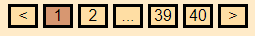
\includegraphics[scale=1]{images/application/pagination.png}
\caption{Navigation és Subnavigation}
\label{fig:pagination}
\end{figure}

A \texttt{Pagination} komponens más komponensekbe egyszerűen implementálható. Pro\-per\-ty-ként meg kell kapnia a jelenlegi oldalt, valamint egy függvényt, ami az oldal változását kezeli. Azt, hogy a találatok közül hanyadik oldalnak kell betöltődnie, az implementáló komponensek tartják számon. Amikor a komponensek lekérik az elemeket az adatbázisból, akkor mellékelniük kell hogy hanyadik oldalt kérik, hogy hogy hány darab találatot kérnek.

\subsubsection{YearSelector komponens}

A \texttt{YearSelector} komponens lehetőséget biztosít, hogy egy lenyíló menüből a felhasználó évszámot választhasson.

\Section{A backend megvalósítása}

A backend \textit{NodeJS} és \textit{Express} segítségével valósul meg. A NodeJS egy nyílt forráskódú JavaScript környezet, amelynek segítségével szerver alkalmazásokat lehet készíteni. Az Express egy minimális és rugalmas NodeJS keretrendszer.

A szerver alkalmazás az Express keretrendszeren kívül más modulokat is felhasznál:
\begin{itemize}
    \item A \texttt{path} modul: Fájl és mappa elérési útvonalakkal való dolgozáshoz ad eszközöket.
    \item A \texttt{morgan} modul: Kérések naplózását végzi.
    \item A \texttt{cookie-parser} és \texttt{body-parser} modulok: Kérések törzseinek és sütijeinek elemzésére használatos.
\end{itemize}

Az útvonalak a \texttt{routes} mappában találhatóak, és az \texttt{index.js} fájlban kerülnek importálásra. A \texttt{config.js} fájlban kerül inicializálásra a Neo4j driver.
